\subsection{Device Physics}\label{device_physics}

\par When transitioning from the traditional static electrical resistor mesh operating in radio frequency from ($f \simeq \SI{30}{\hertz}$, $\lambda \simeq \SI{10000}{k\meter}$) to ($f \simeq \SI{300}{G \hertz}$, $\lambda \simeq \SI{1}{m\meter}$), or microwave frequency from ($f \simeq \SI{300}{M\hertz}$, $\lambda \simeq \SI{1}{\meter}$) to ($f \simeq \SI{300}{G \hertz}$, $\lambda \simeq \SI{1}{m\meter}$) described in Section \ref{electricalPDE} to the Metatronic subwavelength optical frequency domain of ($f \simeq \SI{193}{T\hertz}$, $\lambda \simeq \SI{1550}{n\meter}$) described in Section \ref{metatronicPDE}, control voltage, $V$, in each electrical node is substituted for electric field, $E$ in each Metatronic node. Thus metatronic ‘current’ is not given by the conductivity, but by the displacement current density, $J_D = \frac{\partial D}{\partial t}$, where $D$ is the electric displacement \cite{vakil2011transformation}.

\par The Metatronic circuit board needs to adhere to the condition that $J_D$ is not flowing outside the ‘wire’. This can be realized via biasing a waveguide board to the \acrfull{enz} point, where  $\text{Re}(\varepsilon)$ = real part of permittivity = 0 (or near zero). Here the ‘wire’ is given by regions where $\text{Re}(\varepsilon) >> 0$, termed \acrfull{evl}, where $J_D$ is conducted. 

\Par In order for the metatronic circuit mesh to accurately map to the finite difference equation the physical mesh dimension, $d$, must be much smaller than the optical operation wavelength, $\lambda = \SI{1550}{n\meter}$ (i.e. $d << \SI{1550}{n\meter}$) in order to create the \gls{lumped element model} condition. 

\par In order to duplicate the electrical circuit components resistors, inductors, and capacitors in the metatronic optical subwavelength domain, and in doing so reconfigure the mesh for diffusion and wave equations, the circuit must take advantage of the materials permittivity properties. If the material is a conventional dielectric (e.g., SiO2 or Si) with $\text{Re}(\varepsilon) > 0$ at optical frequencies, the nanoparticle will act as a capacitive impedance (i.e., nano capacitor). If the particle is made of material with $\text{Re}(\varepsilon) < 0$ at optical frequencies (e.g., noble metals such as Ag and Au), the particle may behave as a negatively capacitive impedance, which  implies that it will behave as an inductive impedance (i.e., nano inductor). When the material exhibits some material loss, that is when $\text{Im}(\varepsilon) \neq 0$ (which is almost always the case), a "nano resistor" element should be included in the nanocircuit \cite{N.Engheta_2007}.

\par The \acrshort{enz} materials used is \acrfull{ito} with electrical properties shown in Figure \ref{fig:ITO_material}. The \gls{Drude model} applied to ITO allows one to define optical equivalent circuit models provided the size of the mesh.

\subsection{Finite Difference Equation Equivalence}

\par Following the difference equation mapping in Section \ref{section:electricalDifferenceEquation} through Equation \ref{eq:4} and by sampling displacement current density at each node as well as the node's immediate neighborhood of nodes one edge away, we produce an asymptotically equivalent equation to partial differential equation \ref{eq:electricalLaplace_A} for each Metatronic mesh grid point

\begin{equation}\label{eq:differenceMeta}
  \nabla^2 \varphi \simeq 
  \frac{1}{h^2} \Big[ J_{D1} + J_{D2} +  J_{D3} +  J_{D4} - 4(J_{D0}) \Big].
\end{equation}

\par Equation \ref{eq:differenceMeta} is similar to the application of Kirchhoff's law to the currents $\varphi(P_i)$ meeting at the junction \textit{O} of a lumped circuit mesh described in Equation \ref{eq:voltageSolutionDifferenceLaplace}.

\begin{figure}[ht]
\centering\fbox{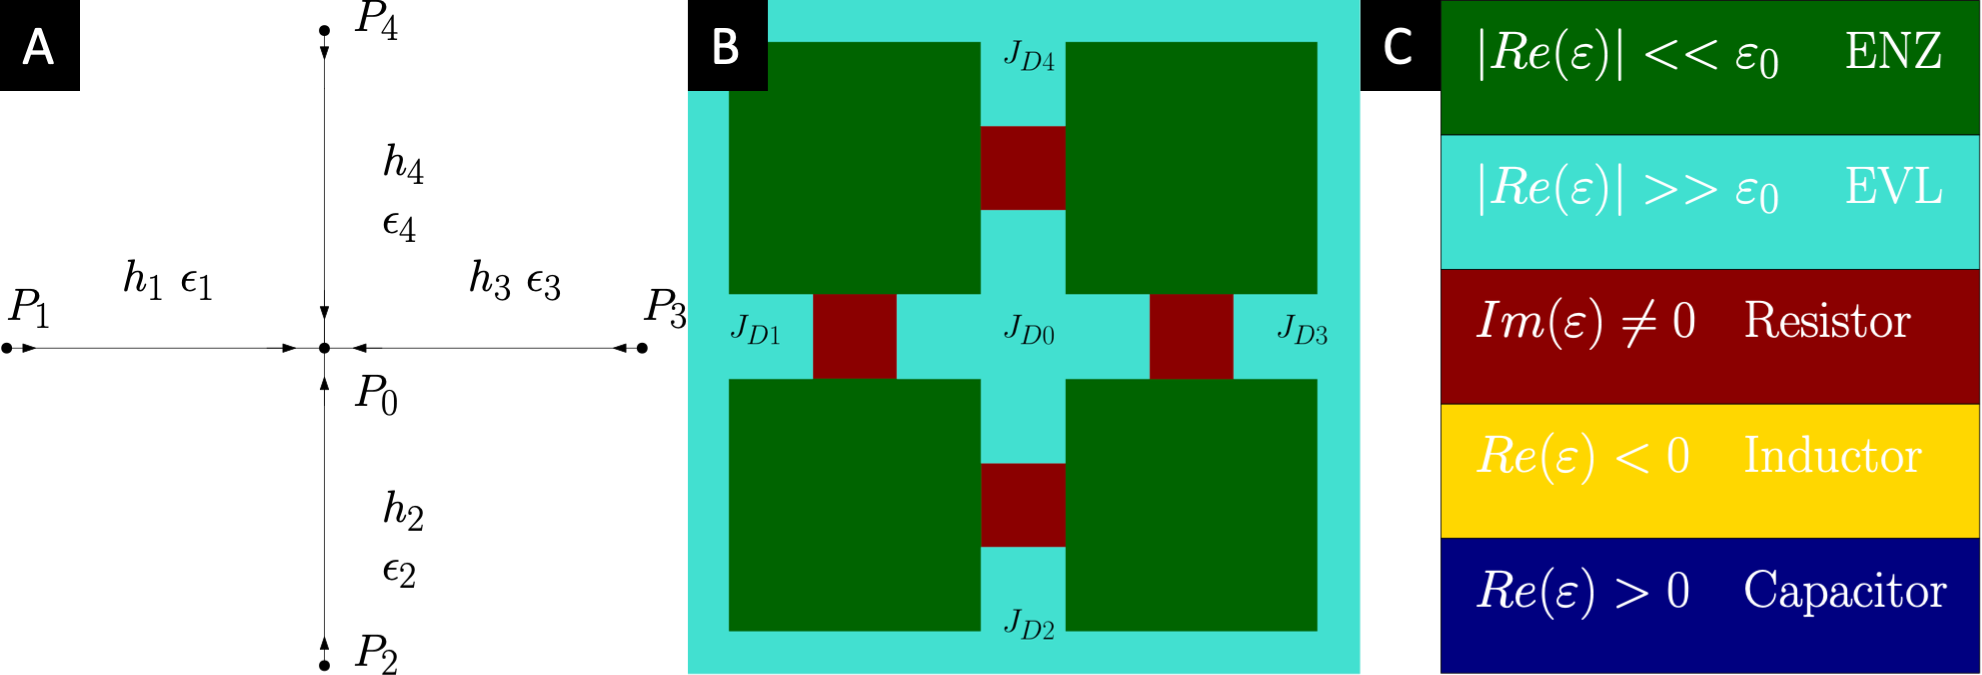
\includegraphics[height=1.5in,width=4.5in]{figures/figures2/05_finite_difference_metatronic.png}}
\caption{The figure shows a \textbf{(A)} finite difference node, a \textbf{(B)} metatronic resistive node with displacement current density sampling locations, and a \textbf{(C)} metatronic material relative permittivity reconfigurability key.}
\label{fig:metaNodeResistive}
\end{figure}

\par An equivalent metatronic nano-optic node is presented in Fig \ref{fig:metaNodeResistive}. 
We exploit the concept that nanoparticles (NPs) in the optics domain can be treated as lumped circuit elements,  whose impedance is defined in terms of the perturbation to the displacement current, $J_D$ in response of the electric field $E$. The materials complex permittivity $\widetilde{\varepsilon}$ acts as a variable for displacement current as follows

\begin{equation}
   J_D = \frac{\partial D}{\partial t} = -j \widetilde{\varepsilon} \omega E(\omega).
   \label{eq:12345}
\end{equation}

\par which, for element size considerably smaller than the optical wavelength [Engheta], represents an equivalent Ohm's law in the optical domain, enabling the mapping of the resistive circuit. In order to convey the flux of the displacement current a sub-wavelength circuit is considered to be carved in an epsilon-near-zero substrate, which for specific optical bandwidth enables light to travel through the grooves just like current in copper wiring \cite{alu2007epsilon}.

\par Resistors, capacitors and inductors can modelled as portions within the air grooves, with materials with well defined permittivity values. In order to map equation \ref{eq:7} in the metatronics circuit, the resistors are modelled as a dissipative dielectric where $R = -j\omega\widetilde{\varepsilon}$ if $\widetilde{\varepsilon}$ is a complex number. 

\par Due to the confinement of the displacement current in the air grooves, the impedances are locally coupled, which in terms of electrical circuit means that a Norton/Thevenin equivalents are admissible. Therefore, for a limited functional bandwidth, for which the material of the board is in ENZ condition, Kirchoff's law at the mesh is satisfied, providing identical results with respect to a resistive network, reported in Equation \ref{eq:differenceMeta}. 

\subsection{\label{sec:PHYSICS3} Solution of Laplace Equation}

\par By following the analytical derivation in Section \ref{section:pdeDerivation} and the electrical mesh mapping in Section \ref{section:electricalDifferenceEquation} as a starting point from which we utilizing COMSOL Multiphyiscs to simulate the electric field displacement and the displacement current in a 3x3 metatronics mesh. A strong local electric field, generated by an horizontal dipole, is used for representing the heat source, while ENZ condition is applied to the rest of the boundaries. In this section, as an illustrative and not limiting, example the permittivity of the circuit board is considered to have negligible losses ($\varepsilon''<0.1$) ($\widetilde{\varepsilon}\simeq0$) with an overall size of 1000 nm ($d<\lambda$) \cite{moitra_experimental_2014, li_-chip_2015}.

\par The overall dimension of the circuit of Fig. \ref{fig:photonic_metatronic_simulations}C is supposed to be smaller than the operating wavelength, as required for conventional electronic circuit concepts at low frequencies. However, the ‘‘spatially static-like’’ properties of the ENZ substrate, i.e. absence of a significant phase variation in ENZ, essentially relax this requirement for the optical nano-circuit board of Fig. \ref{fig:metatronic_size_simulation}, for which the total length may become also several free-space wavelengths long (while it is electrically small compared to the very long wavelength in ENZ).\cite{li_-chip_2015}

\par Under these conditions, the field lines in Figure \ref{fig:metatronic_size_simulation} highlights that the Electric displacement and consequently the displacement current, fall only within the air grooves, forced by the ENZ conditions in the neighboring area ($D\simeq0$). 

\par These COMSOL Multiphyics simulations, with maximum computational mesh size of \SI{5}{n\meter}, of electric displacement field, with $\lambda \approx \SI{1550}{n\meter} $ and $f \approx \SI{193}{T\hertz}$, over \acrfull{ito},  with complex permittivity $\epsilon = 1.0e-4 + i0.3$, in \acrfull{enz} condition squares in subwavelength optical regime surrounded by air channels, with a width of $\SI{10}{n\meter}$, broken by metatronic resistive $\SI{10}{n\meter} \times \SI{10}{n\meter}$ squares composed of \acrshort{ito} with complex permittivity $\epsilon = 1.0e-4 + i0.3$ squares described in section \ref{device_physics}. The simulation applies an initial electrical field along the top of each array with a value of $\SI{1}{\volt\meter}$ with scattering boundary conditions applied to the remaining three sides of each array. The electrical displacement current density (shown as white arrows), used to sample the \acrshort{pde} solution from the grid, is confined to the air groves surrounding and throughout the mesh.

\begin{figure}[ht]
\centering\fbox{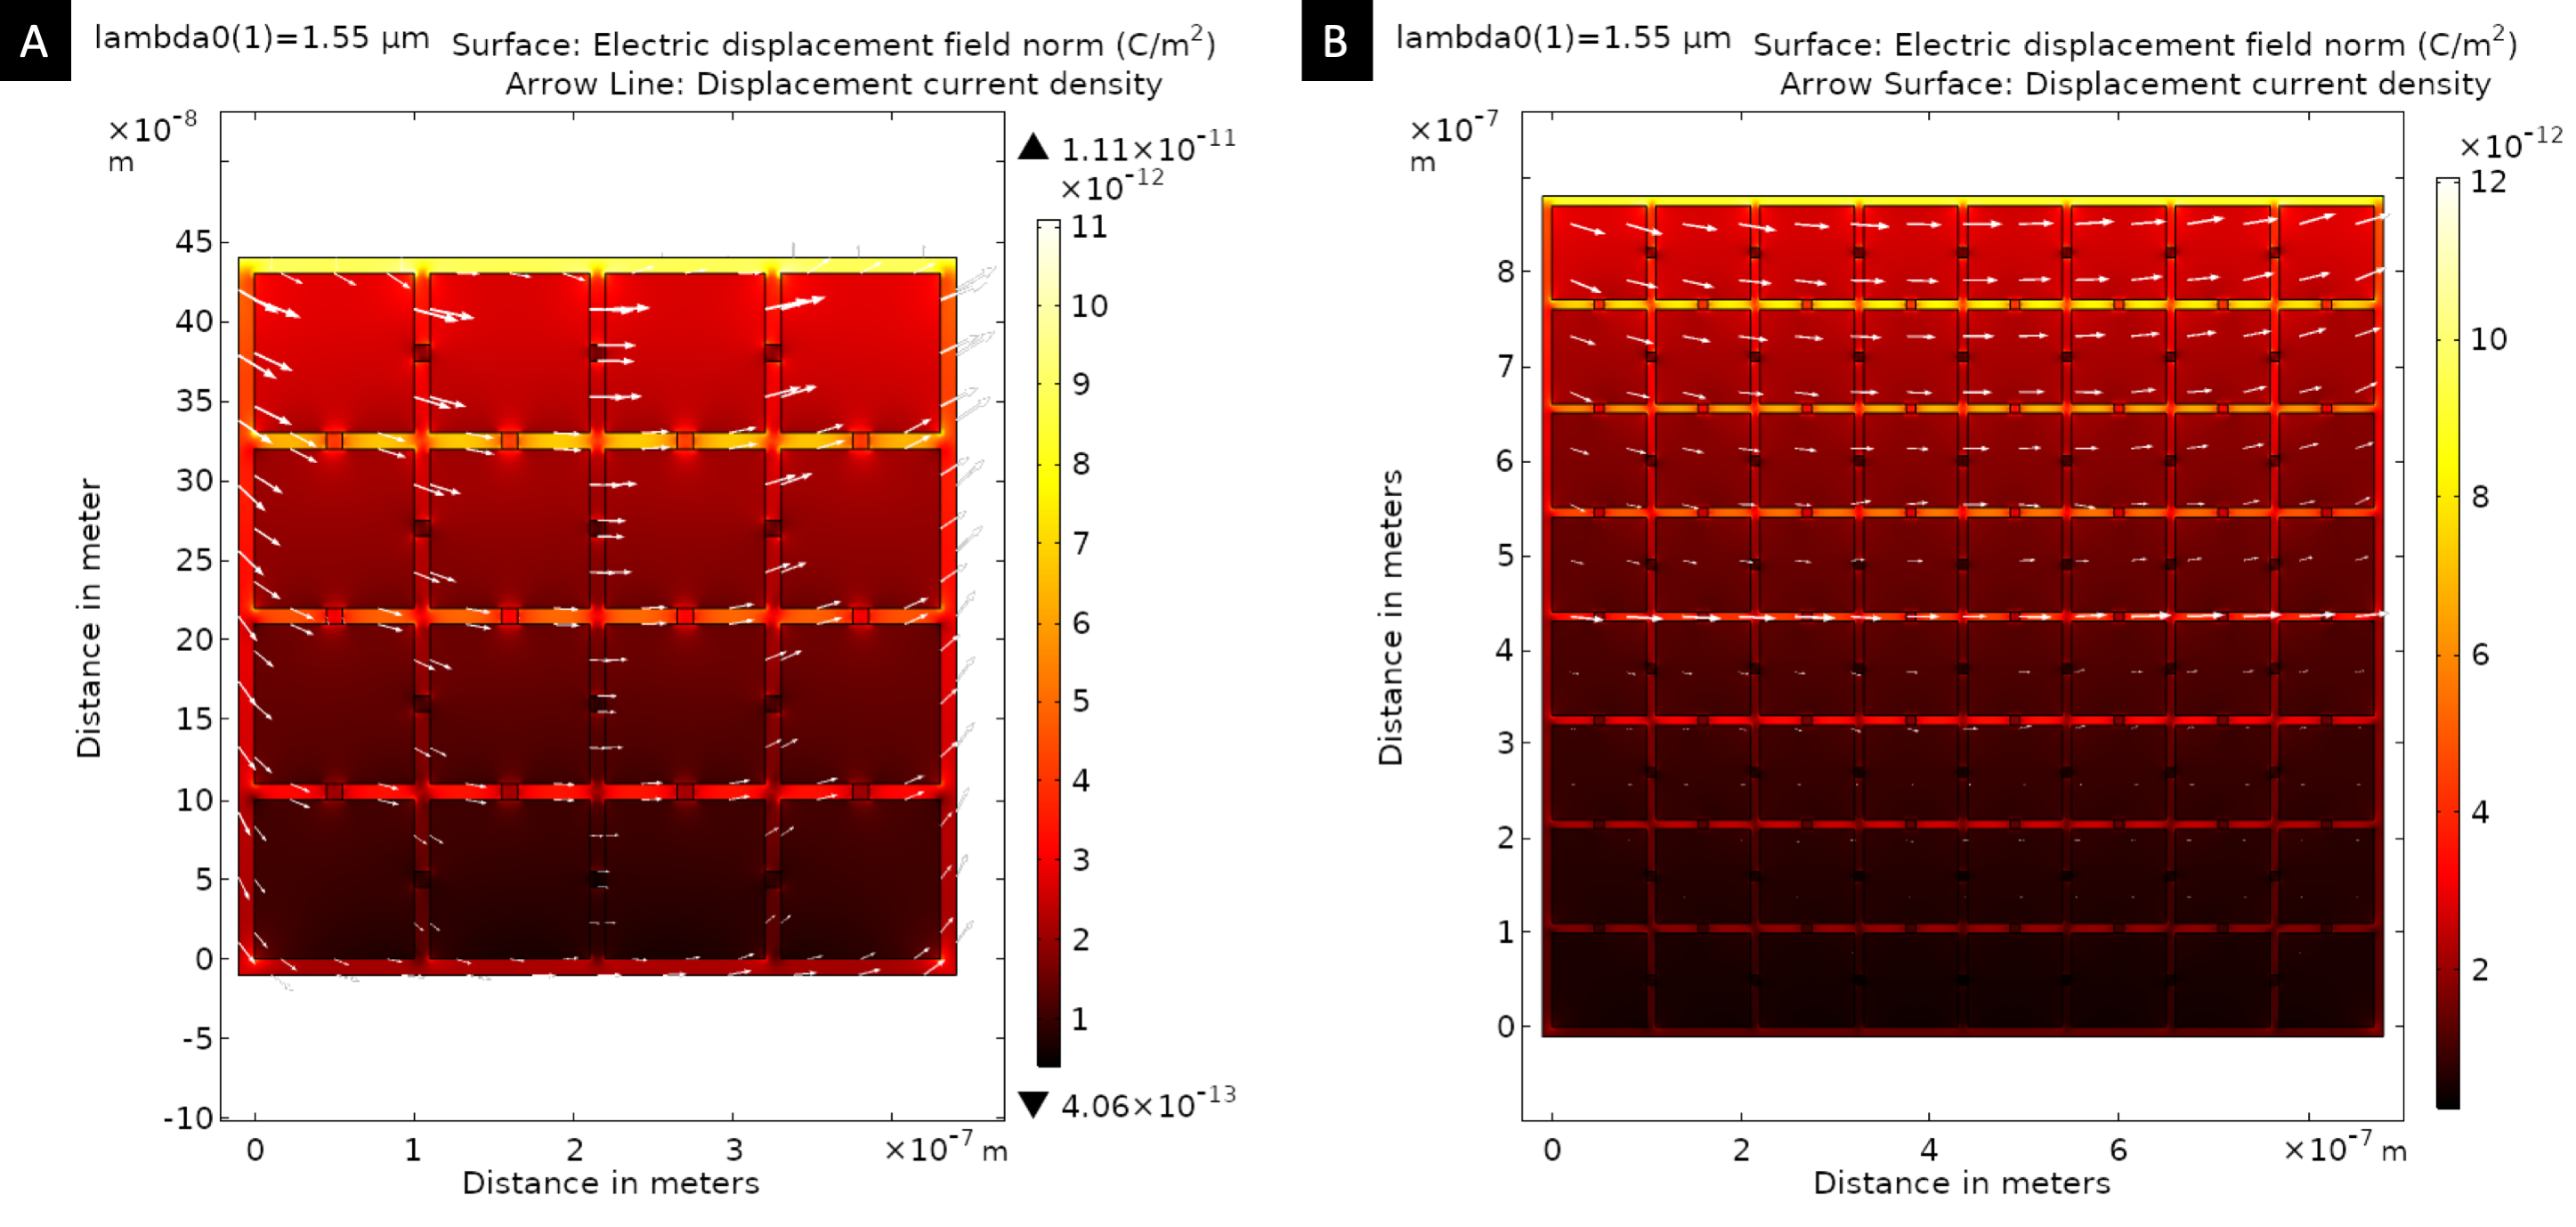
\includegraphics[width=5.5in]{figures/figures2/11_mt4_and_mt8.png}}
\caption{The \acrfull{enz} boxes in this simulation are $\SI{100}{n\meter} \times \SI{100}{n\meter}$ and the \acrfull{evl} groves are $\SI{10}{n\meter}$ wide where \textbf{(A)} contains 4 by 4 \acrshort{enz} boxes and \textbf{(B)} contains 8 by 8. One can see that at longer length scales the electric displacement field continues to produce the form of the \acrshort{pde} solution, but the containment of displacement current density within the \acrshort{evl} air groves is weakened.} 
\label{fig:metatronic_size_simulation}
\end{figure}

\par Solutions of the PDE solving metatronic processor with increasing mesh density are reported in Figure \ref{fig:metatronic_accuracy}. Interestingly, the solution given by the metatronic circuit for increasing mesh densities, keeping the overall circuit dimension, maps precisely the solution of a finer mesh in a finite difference approach.  This is can be achieved only if the circuit board is characterized by negligible losses, which causes the absence of a dielectric field displacement in the ENZ circuit board providing a perfect electric-circuit behavior. 

\par However, a study of the size and scalability and their impact on the accuracy of the solution of the metatronic processor becomes absolutely determinant if the losses in the ENZ circuit board are not negligible as discused in Section \ref{sec:ITO}). Other parameters, such as width of the grooves and smoothness of the bending curves can impact the accuracy of the solution. The undesired influence of these parameters, here not discussed,  would results in a systematic error that can be compensated or mitigated by accurate and controlled processes.

\subsection{\label{sec:ITO}  Monolythic Integration}

\begin{figure}[ht]
\centering\fbox{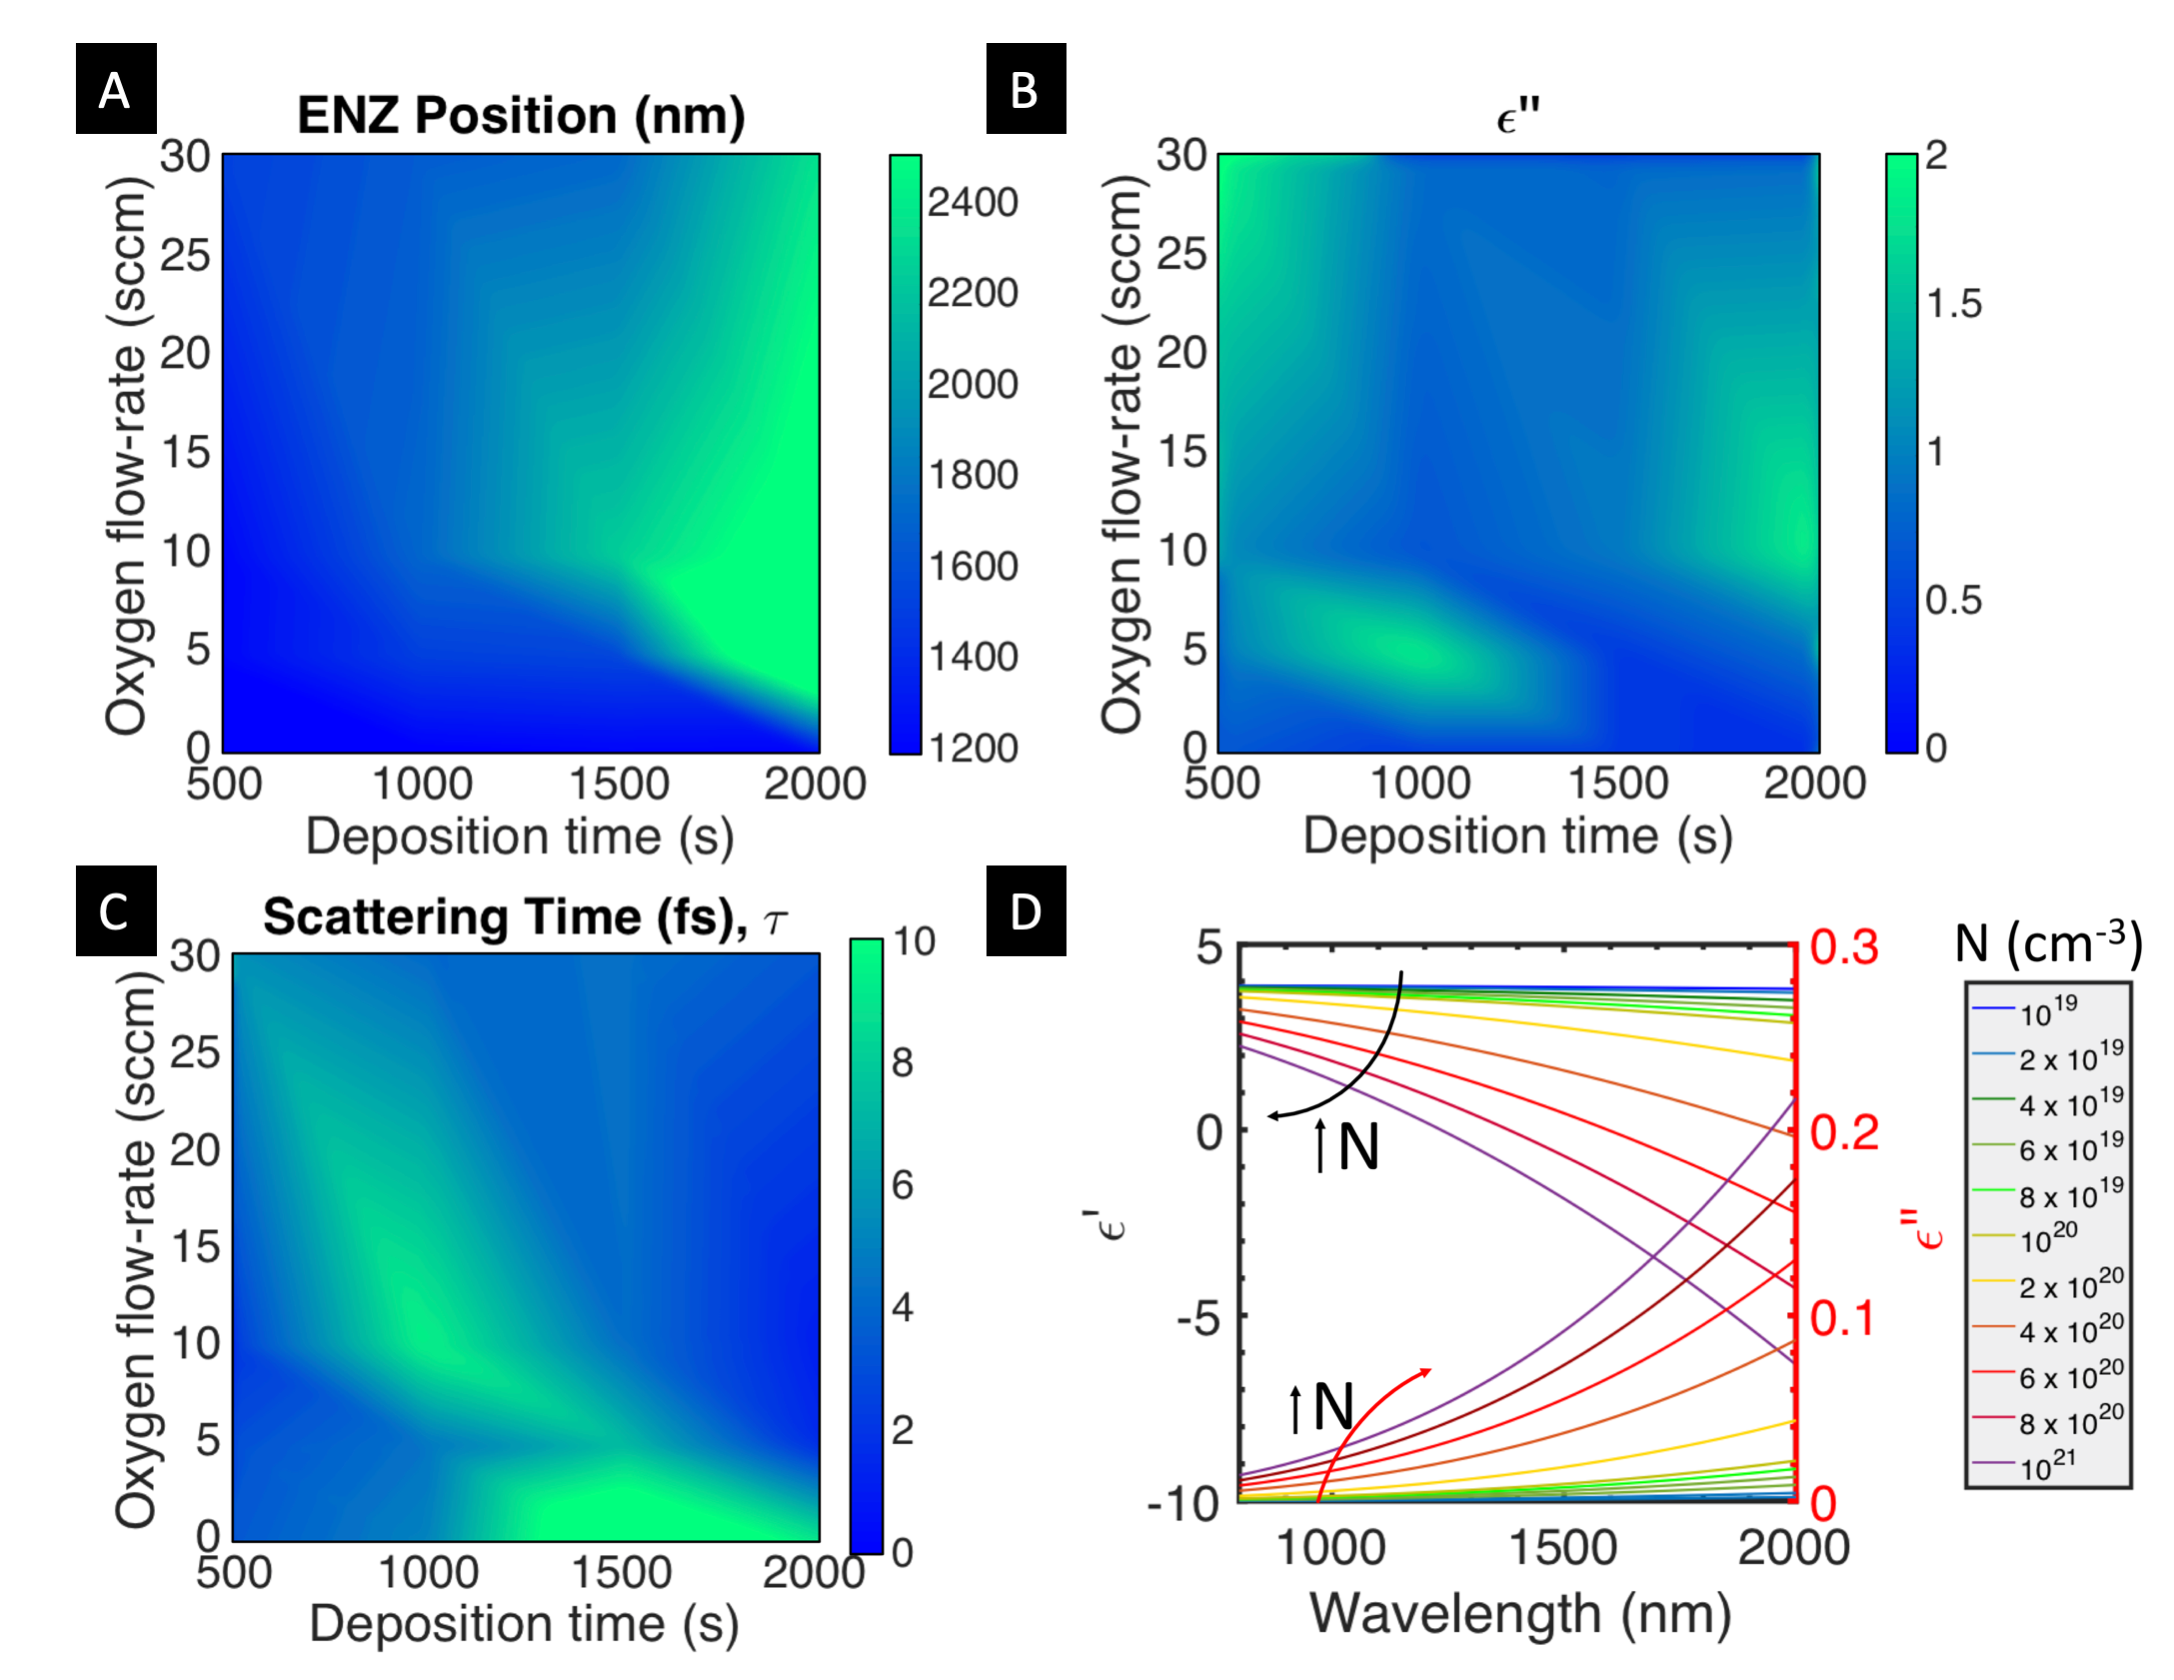
\includegraphics[width=5in]{figures/figures2/12_ito_material_new.png}}
\caption{The \textbf{(A)} ENZ wavelength, \textbf{(B)} Electrostatic doping, and \textbf{(C)} Scattering Time ($\tau_{sc}$) as function of process parameters (Oxygen flow-rate and deposition time). The  \textbf{(D)} Drude model of ITO film, sputtered with an initial electron doping of $10^{19}$cm$^{-3}$ and $\Gamma= \frac{1}{\tau_{sc}}$, for an increasing carrier modulation (blue to red).}
\label{fig:ITO_material}
\end{figure}

\par In the past years, few materials have been considered for fabricating a metatronic circuit board, such as multilayered stacks of thin film \cite{Lie1501790,PhysRevApplied.10.054021} , NPs assemblies and graphene. However, their large-scale integration is far from easy.

\par We propose Indium tin oxide as suitable material for a monolithic integration of the proposed metatronic processor. ITO has a tunable and controllable ENZ position in the NIR, according to process parameters (e.g. Oxygen flow-rate, Thermal Annealing). Its optical properties, imaginary and real part of the permittivity, can be electrostatically tuned \cite{sorger_ultra-compact_2012,amin_0.52_2018}, thus allowing GHz fast\cite{dalir_atto-joule_2018} energy efficient \cite{amin_attojoule_2018} reprogrammable features on the circuit board. 

\par Moreover, recently, our group achieved a consistent control over ITO optical parameters in particular with respect to the ENZ wavelength as function of sputtering parameter, thus allowing to bridge the technological gap in the implementation of metatronic circuits \cite{gui2018impact}. According to our fundamental studies, depicted in figure \ref{fig:ITO_material}, the ITO for the ENZ circuit board is supposed to be sputtered with 5 sccm Oxygen flow rate, enabling a 200 nm film in ENZ condition at 1550 nm, with not negligible losses $\widetilde{\varepsilon}= 0.3i$ which corresponds to a scattering time, $\Gamma= 2$ fs. The resistors, deposited using 20 sccm oxygen flow rate, which yields to $\widetilde{\varepsilon}=1.2+0.8i$  and a scattering time of 5fs. 

\par The major disadvantage is represented by the losses at ENZ condition. As a consequence of the losses in the ITO circuit board, the lines of the displacement field are not only contained in the air grooves, contrarily to the case of a ENZ material with negligible losses. In presence of non-negligible losses in the ENZ material, the circuit board is not completely insulating, since the displacement current is not negligible.

\begin{equation}
     J_D = \frac{\partial D}{\partial t}=\varepsilon"\omega E(\omega).
\end{equation}

\par There are two major kinds of phenomena that impact the accuracy of the solution, both of which depend on the ITO losses. The first one, is a function of the mesh density and the second one of the total physical length of the circuit board. High density ($>5\times5$) induces coupling within wires that shouldn't be connected, while the larger physical length ($>2\mu$m) contributes to unwanted dissipation, deviating from the original solution.

\par Figure \ref{fig:metatronic_accuracy} plots the accuracy as function of the number of nodes and physical dimension of the circuit board. The maximum accuracy ($>90$\%) is obtained for a $1\mu$m grid, with a $4\times4$ mesh density. This is achieved thanks to the trade-off between mesh size and density, which minimizes the wire coupling, without extending the wiring length, producing unwanted losses. 

\par The ITO is considered to be in a capacitor configuration, spaced by a thin dielectric, for electrostatic doping, enabling fine tuning of the permittivity values as well as updating of the problem. 

\par The variation of the carrier density via gating in ITO affects both the resistance and the ``reactance''  in the metatronics equivalent circuit, hindering the accuracy of the solution, being Imaginary, and the real part of the permittivity in Kramer-Kronig relation. Nevertheless, contrarily to the resistive circuit, if either the boundary conditions or the impedances are quickly ``refreshed'', the nano-optics equivalent circuit is substantially not affected by dispersion. In this case, the lumped circuit model still holds for high frequency modulation, since even at 100s of GHz, the timescale at which the signal is modulated does so substantially slower than the time taken by the optical signal to travel through the nano-optics network.

\subsection{\label{sec:Performance} ITO based Performance}

\begin{figure}[ht]
\centering\fbox{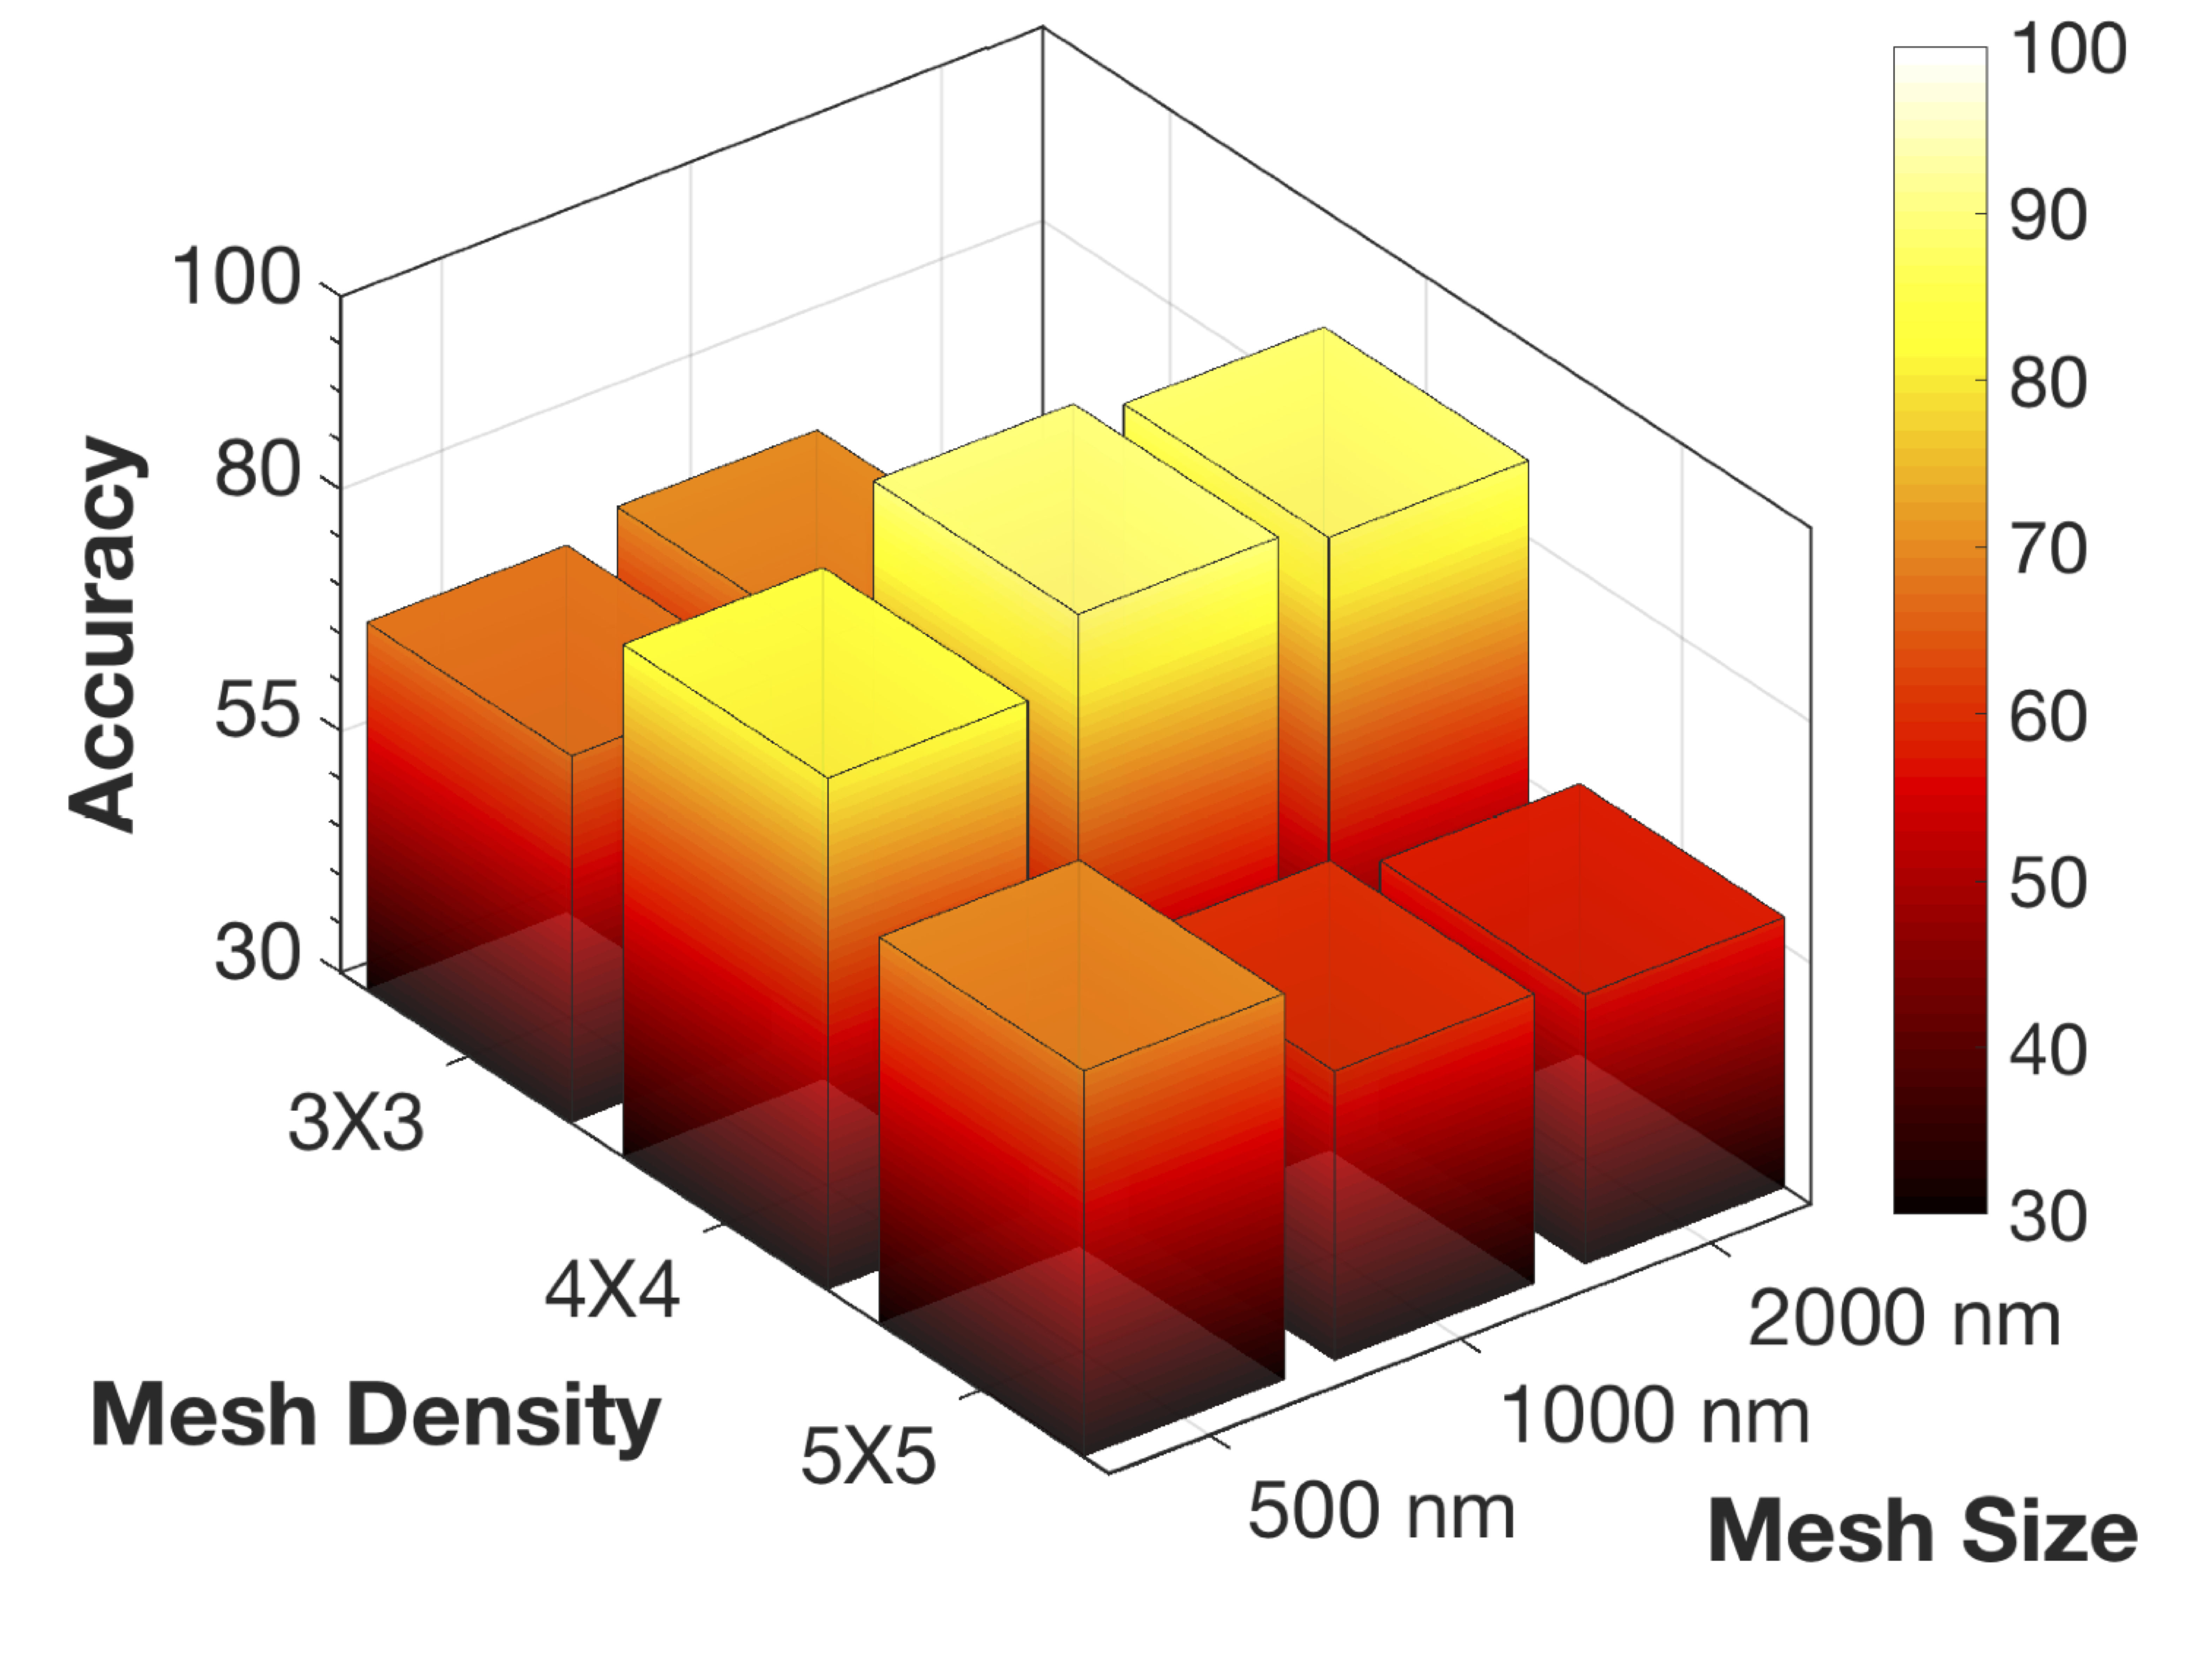
\includegraphics[width=5in]{figures/figures2/14_ito_performance_b.png}}
\caption{The metatronic solution accuracy as function of mesh density and size when compared to an discrete \acrshort{pde} solution.}
\label{fig:metatronic_accuracy}
\end{figure}

\par The main limitation of the ITO metatronic processor are the unwanted losses in the circuit board. The losses affect both the power consumption and the accuracy of the solution. However, for a small size of the processor, an approximate solution is given. The accuracy is shown in terms of error computed with respect to the solution of a finite difference of comparable mesh density.

\par The power consumption from the processor is the summation of the optical power used for exciting the dipole (initiating the processor) and the the radio frequency power employed for modulating the carrier densities of each lumped elements, i.e. reprogramming the circuit. Concerning the reconfigurability of the processor, recent works showed attojoule efficient \cite{amin_attojoule_2018,dalir_atto-joule_2018} ITO based modulators operating at high speed. On the other hand, few mW optical power are needed for exciting the fluorescent molecule and setting the boundary conditions. Although, efficient measurements schemes must be used for detecting the electric field displacement at each node of the metatronic mesh, avoiding scanning over the sample, e.g. high resolution tip enhanced near field spectroscopy, in order to minimize the power used for the detection mechanism.

\subsection{\label{sec:Probe} Near Field Displacement Measurement}

\begin{figure}[h]
\centering\fbox{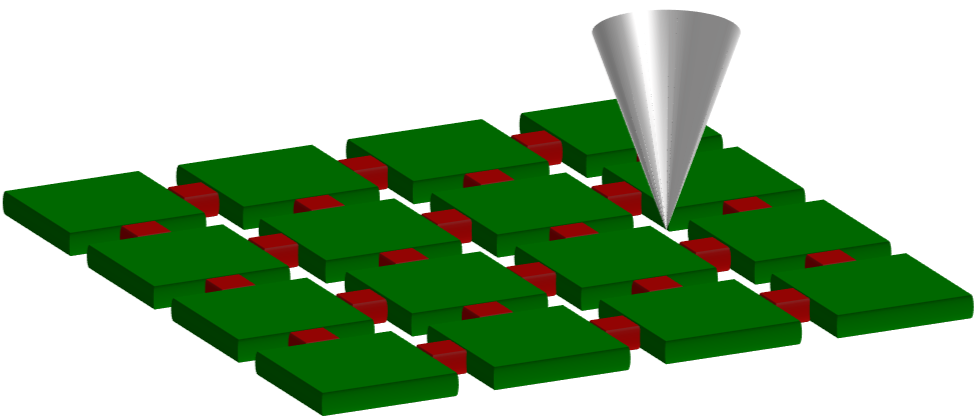
\includegraphics[width=4in]{figures/figures2/15_probetip.png}}
\caption{Schematic representation of a "Nanophotonic Probe". An impinging radiation excites a fluorescent molecule, creating a local near field, which produces an electric displacement in the metatronic circuit. The displacement is probed by the tips of a probe card, in a campanile tip aperture nSOM configuration.}
\label{fig:nanophotonic_probe}
\end{figure}

\par In order to sample the electric field displacement signal at the nodes of the metatronic mesh, deep sub-wavelength near field microscopy has to be employed with nanometric spatial resolution \cite{bao_mapping_2012,bao_visualizing_2015,caselli_deep-subwavelength_2015}. Although, regular Near-field is associated with AFM systems, thus requiring long scanning time. In this section, we propose a Nano-optic probe card for reading of the values of the local displacement field as shown in Figure \ref{fig:nanophotonic_probe}). The reading mechanism is based on multiple tips characterized by sub-wavelength aperture at the apex which collects the local near field radiation similarly to a local near field microscope, allowing for a parallel reading out. NSOM would be preferential with respect to Scattering type SNOM since the former will minimize the coupling between vertical dipoles, i.e. metallic tip, introducing second order scattering and a higher degree of uncertainty in the system.


